% Draft paper. Compile on Overleaf (New Project -> Upload Project -> this folder's zip).
% Everything marked \TODO{...} needs your real results or your own wording.
% DO NOT submit any number you did not produce by running the benchmark.
\documentclass[conference]{IEEEtran}
\usepackage{booktabs}
\usepackage{graphicx}
\usepackage{xcolor}
\usepackage{hyperref}
\newcommand{\TODO}[1]{\textcolor{red}{[TODO: #1]}}
\graphicspath{{../results/figures/}{figures/}}

\begin{document}

\title{How Much Do Logs Matter? Evaluating LLM Root-Cause Analysis Under Degraded Observability With Controlled Fault Injection}

\author{\IEEEauthorblockN{Prisha \TODO{surname}}
\IEEEauthorblockA{Department of Computer Science and Engineering\\
SRM Institute of Science and Technology, Ramapuram, Chennai, India\\
\TODO{email}}
\and
\IEEEauthorblockN{\TODO{Faculty guide}}
\IEEEauthorblockA{\TODO{Department, SRM IST}}}

\maketitle

\begin{abstract}
Large language models (LLMs) are increasingly proposed as assistants for diagnosing production incidents, but most evaluations use real incident archives whose ground truth is uncertain and whose evidence quality cannot be controlled. We present a reproducible benchmark that injects eight realistic faults (database, payment-provider, resource, deployment, cache and storage failures) plus no-incident controls into a simulated web service, and renders each incident under four observability conditions: full logs, noisy logs with misleading distractors, generic logs without causal detail, and metrics only. Because every condition is derived from the same underlying trial, differences between conditions are paired comparisons on identical incidents. We evaluate \TODO{N} LLMs against a hand-tuned expert runbook and a chance baseline on 480 evidence bundles. \TODO{One sentence with the main finding, e.g. how much accuracy drops from full logs to metrics only, and whether larger models are more robust.} \TODO{One sentence on calibration or false alarms.} The benchmark, dataset and evaluation code are released to support reproducible research.
\end{abstract}

\begin{IEEEkeywords}
root cause analysis, large language models, AIOps, observability, fault injection, site reliability engineering
\end{IEEEkeywords}

\section{Introduction}
When a production service degrades, on-call engineers must decide quickly \emph{why}. They combine an alert, metric dashboards, recent changes and log lines into a diagnosis. LLMs can read all of these modalities as text, which has motivated their use for automated root-cause analysis (RCA) \TODO{cite LLM incident RCA work, see references-to-verify.md}.

Evaluating such systems is hard. Real incident archives rarely have certain ground truth, and the quality of the available evidence varies in ways that cannot be controlled. In particular, it is unclear how much an LLM's diagnosis depends on \emph{descriptive} log messages (for example ``database connection timeout''), and how it behaves when logs are noisy, generic or missing. This is common in practice: logging is often sparse, inconsistent or sampled.

We address this with controlled fault injection, in the spirit of chaos engineering \TODO{cite}. We make three contributions:
\begin{itemize}
  \item A reproducible RCA benchmark: a simulated e-commerce service with a catalogue of eight faults and no-incident controls, rendered under four paired evidence conditions (Section~\ref{sec:bench}).
  \item An evaluation of \TODO{N} LLMs, including small models that run locally, against an expert rule baseline, measuring accuracy, robustness, multi-fault diagnosis, false alarms and calibration (Section~\ref{sec:setup}).
  \item An analysis of which faults and evidence conditions cause failures, with paired significance tests (Section~\ref{sec:results}).
\end{itemize}

\section{Related Work}
\TODO{Write 3 short paragraphs in your own words, each citing papers you have actually read:
(1) LLMs for cloud incident management and RCA;
(2) traditional AIOps RCA from metrics, logs and traces, and existing RCA benchmarks;
(3) chaos engineering and fault injection.
End with one sentence on what is different here: controlled, paired evidence-quality conditions with exact ground truth.}

\section{Benchmark}
\label{sec:bench}
\subsection{Simulated service}
The system under test is \emph{shop-api}, a FastAPI service with product listing and detail endpoints (served from a cache, falling back to a database), a checkout endpoint (database, external payment provider, then a receipt written to local storage), and a health endpoint. A load generator issues a realistic mix of requests (45\% listing, 27\% detail, 25\% checkout, 3\% health). The service uses real routing, middleware, HTTP status codes and structured logging; only waiting is simulated, using a virtual clock. Each request accumulates simulated latency instead of sleeping, so a four-minute trial runs in well under a second and is exactly reproducible from its random seed.

\subsection{Fault catalogue}
Table~\ref{tab:faults} lists the injected faults. They were chosen to include pairs that are easy to confuse from coarse metrics alone. For example, a bad deployment and a full disk both produce HTTP 500 errors on checkout only, and a slow database and a saturated CPU both raise latency without errors. Control trials inject no fault but double the traffic, which trips a traffic alert; the correct answer is \texttt{no\_incident}.

\subsection{Trials and evidence conditions}
Each trial runs a 120-second baseline window, then injects its faults (and, in half of the trials, records a harmless change such as an unrelated deployment, as a red herring) and runs a 120-second incident window. From each trial we derive one \emph{evidence bundle} per condition:
\begin{itemize}
  \item \textbf{Full}: all warning and error logs from the incident window.
  \item \textbf{Noisy}: about 15\% of the real log lines, mixed with three times as many plausible distractors, some of which deliberately implicate the wrong component.
  \item \textbf{Generic}: log lines reduced to the failing status code and path, with no causal text.
  \item \textbf{Metrics only}: no logs.
\end{itemize}
All bundles contain the same alert, per-endpoint metrics (request rate, 5xx rate, p50 and p95 latency for both windows), status-code counts, CPU utilisation, service version and recent changes. Because the four bundles of a trial share identical metrics, comparisons across conditions are paired.

The dataset contains 80 single-fault trials (10 seeds per fault), 20 two-fault trials and 20 controls, giving 480 bundles. The trial plan is derived from a fixed master seed.

\section{Experimental Setup}
\label{sec:setup}
\subsection{Methods}
\textbf{LLMs.} \TODO{List each model with provider, size and exact version string, and the date you ran it.} All models receive the same system prompt, which describes the architecture and the nine allowed labels and asks for a JSON answer with a root cause, an optional secondary cause, the faulty component, a confidence in $[0,1]$ and a short explanation. Temperature is 0. Unparseable answers or labels outside the set count as incorrect.

\textbf{Expert runbook (rules).} Keyword rules over logs, then metric patterns (version change, CPU, which endpoints fail or slow down, gateway status codes). It was written with knowledge of the fault catalogue, so it is a strong upper reference rather than a fair competitor; its role is to show how much of the task is solvable by an engineer with full knowledge of the system.

\textbf{Majority.} Always predicts one label; the chance floor.

\subsection{Measures}
Accuracy on single-fault and control bundles with 95\% Wilson intervals; macro-F1 over labels; component accuracy; for two-fault trials, whether the primary answer is one of the true causes and whether both are named; false-alarm rate on controls; invalid-output rate; expected calibration error (ECE, 10 bins); and mean latency and tokens per call. Differences between methods on the same bundles are tested with the exact McNemar test.

\section{Results}
\label{sec:results}
% Auto-generated by `python -m rcabench report`. Do not edit by hand.
\begin{table}[t]
\centering
\caption{Root-cause accuracy (\%) by evidence condition.}
\label{tab:accuracy}
\begin{tabular}{lrrrrr}
\toprule
Method & Full logs & Noisy logs & Generic logs & Metrics only & Overall \\
\midrule
majority & 10.0 & 10.0 & 10.0 & 10.0 & 10.0 \\
rules & 100.0 & 74.0 & 90.0 & 90.0 & 88.5 \\
\bottomrule
\end{tabular}
\end{table}

\begin{table}[t]
\centering
\caption{Secondary measures (\%, except ECE).}
\label{tab:secondary}
\begin{tabular}{lrrrrr}
\toprule
Method & Component & Multi-fault hit & False alarm & Invalid & ECE \\
\midrule
majority & 36.0 & 50.0 & 100.0 & 0.0 & 0.011 \\
rules & 92.5 & 97.5 & 22.5 & 0.0 & 0.266 \\
\bottomrule
\end{tabular}
\end{table}

\begin{table}[t]
\centering
\caption{Fault catalogue (ground-truth labels).}
\label{tab:faults}
\begin{tabular}{p{0.3\linewidth}p{0.6\linewidth}}
\toprule
Label & Injected behaviour \\
\midrule
bad\_deployment & New release 1.4.0 has a bug: ~60\% of checkouts raise an unhandled KeyError. \\
cache\_failure & Cache cluster refuses connections; reads fall back to the database (slower, no errors). \\
database\_outage & Database unreachable: queries hang until a connection timeout, requests fail with 503. \\
database\_slow & Database degraded: queries take 0.5-2 s, occasional slow-query warnings, no errors. \\
disk\_full & Receipt volume is full: ~50\% of checkouts fail writing receipts (ENOSPC). \\
resource\_saturation & Service CPU saturated: every endpoint (including /health) slows down uniformly. \\
upstream\_payment\_errors & Third-party payment provider returns 502 for ~40\% of charges. \\
upstream\_payment\_slow & Payment provider responds in 1.5-4 s; calls over 3.5 s time out with 504. \\
no\_incident & Control: harmless 2.2$\times$ traffic spike, nothing broken \\
\bottomrule
\end{tabular}
\end{table}


\begin{figure}[t]
\centering
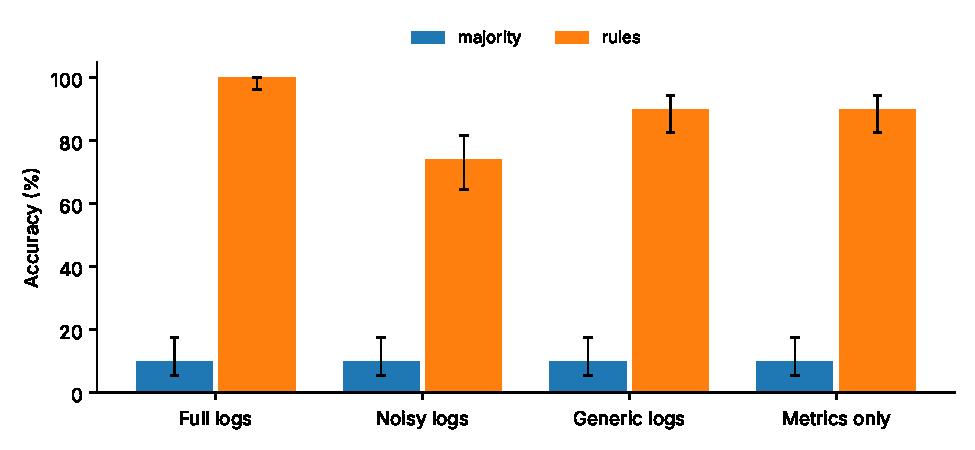
\includegraphics[width=\linewidth]{accuracy_by_condition.pdf}
\caption{Accuracy by evidence condition, with 95\% Wilson intervals.}
\label{fig:conditions}
\end{figure}

\TODO{Describe Table~\ref{tab:accuracy} and Fig.~\ref{fig:conditions}: overall ranking; the drop from Full to each degraded condition for each model; whether noisy logs (misleading evidence) hurt more than missing logs. Quote McNemar p-values from results/summary.md.}

\TODO{Per-fault analysis using the confusion matrices in results/figures: which pairs get confused (expected: bad\_deployment vs disk\_full, database\_slow vs resource\_saturation), and whether models use the version change and CPU metric when logs are absent.}

\TODO{Multi-fault, false alarms on controls, calibration (are wrong answers given with high confidence?), cost and latency.}

\section{Discussion}
\TODO{What should practitioners take away? For example, whether investing in descriptive logs matters more than model size, and whether confidence can be trusted for auto-remediation. Keep claims within what your numbers show.}

\section{Threats to Validity}
\textbf{Simulation realism.} The service and faults are simplified; real incidents involve more components, traces and cascading effects. We mitigate this by using a real web framework and realistic log text, but results may not transfer directly to production systems.
\textbf{Label leakage into the prompt.} The prompt lists all nine labels with short descriptions, which makes the task a constrained classification. Open-ended RCA is harder.
\textbf{Rule baseline.} The rules were tuned with knowledge of the faults, so their accuracy is optimistic.
\textbf{Model drift.} Hosted models change over time; we report model versions and run dates and release all predictions.
\textbf{Scale.} \TODO{Number of seeds per fault; consider more seeds if confidence intervals are wide.}

\section{Conclusion}
\TODO{Two or three sentences restating the question, the main finding and the released artefact.}

\section*{Availability}
Code, dataset generator and all model predictions: \TODO{GitHub URL}.

% Add a references.bib exported from Google Scholar (use the "Cite -> BibTeX" link)
% for each paper you actually read, then uncomment:
% \bibliographystyle{IEEEtran}
% \bibliography{references}

\end{document}
